\section{Microsoft Kinect}
En Kinect er et Natural User Interface (NUI) udviklet til Microsoft's spillekonsol, Xbox.
Den gør det muligt at interagerer med sin konsol ved at bevæge kroppen og via talte kommandoer.
Den første version der udkom i november 2010\cite{kinectWiki} er oprindeligt udviklet med henblik på at lokke nye typer brugere til Xbox med det argument at det via naturlig (og aktiv) bevægelse er sjovere og mere virkelighedstro at spille.

Dog blev der i februar 2012 lanceret en ny type Kinect, kaldet Kinect for Windows, der der sammen med et Software Development Kit (SDK) gør det muligt at udvikle både kommercielle og non-kommercielle applicationer til Kinect som også kan eksekveres på Windows platformen.
Kort fortalt er Microsoft's Kinect mere end en input enhed gamere kan bruge for at gøre deres spiloplevelse mere virkelighedstro; af andre anvendelser kan f.eks. nævnes\cite[s.~17]{kinectProgrammingGuide}:

\begin{itemize}
\item Optagelse af video i real-tid
\item Måle afstand mellem objekter og deres omgivelser
\item Generere et dybde billede ved hjælp af kameraet og de to IR sensorer
\item Sende talte kommandoer
\item Vurdering af omgivelserne ved hjælp af lyd
\end{itemize}

Dette er alle interessante eksempler der på hver deres måde kan afhjælpe problemet med at bestemme en autonom robots placering i ukendte omgivelser.
Derfor vil Kinecten, både med hensyn til hardware, men også til software blive nærmere beskrevet i de følgende afsnit.


\subsection{Opbygning af Kinect}
\textbf{A Prime Sense PS1080-A2.
"Kinect is based on Prime Sense's motion detection technology," explains Kyle.
"This chip is the Kinect's brains —– all the sensors are wired into here for processing before transmitting a refined depth map and color image to the Xbox."}

I denne rapport er det versionen Kinect for Windows der beskrives, da den er tilgængelig gennem universitetet.

Dog kan det nævnes at forskellene mellem den og versionen til Xbox er meget små.
Hardware mæssigt har Kinect for Windows den fordel at firmwaren indeholder en såkaldt Near Mode, hvilket gør det muligt at følge objekter indtil 40 cm fra enheden.

Kinect for Xbox har ikke denne funktionalitet, og kan derfor kun følge objekter indtil 80 cm fra enheden.
Kinect for Windows kan desuden også benyttes til kommercielle applikationer, hvor dens pendant er beregnet til hobbyister, generel udvikling og forskning\cite[s.~16]{kinectProgrammingGuide}.

For at Kinecten kan følge et objekt kræver det selvfølgelig noget specifikt hardware, som overordnet set består den af nogle sensorer, et farve kamera samt nogle mikrofoner.

\begin{figure}
\centering
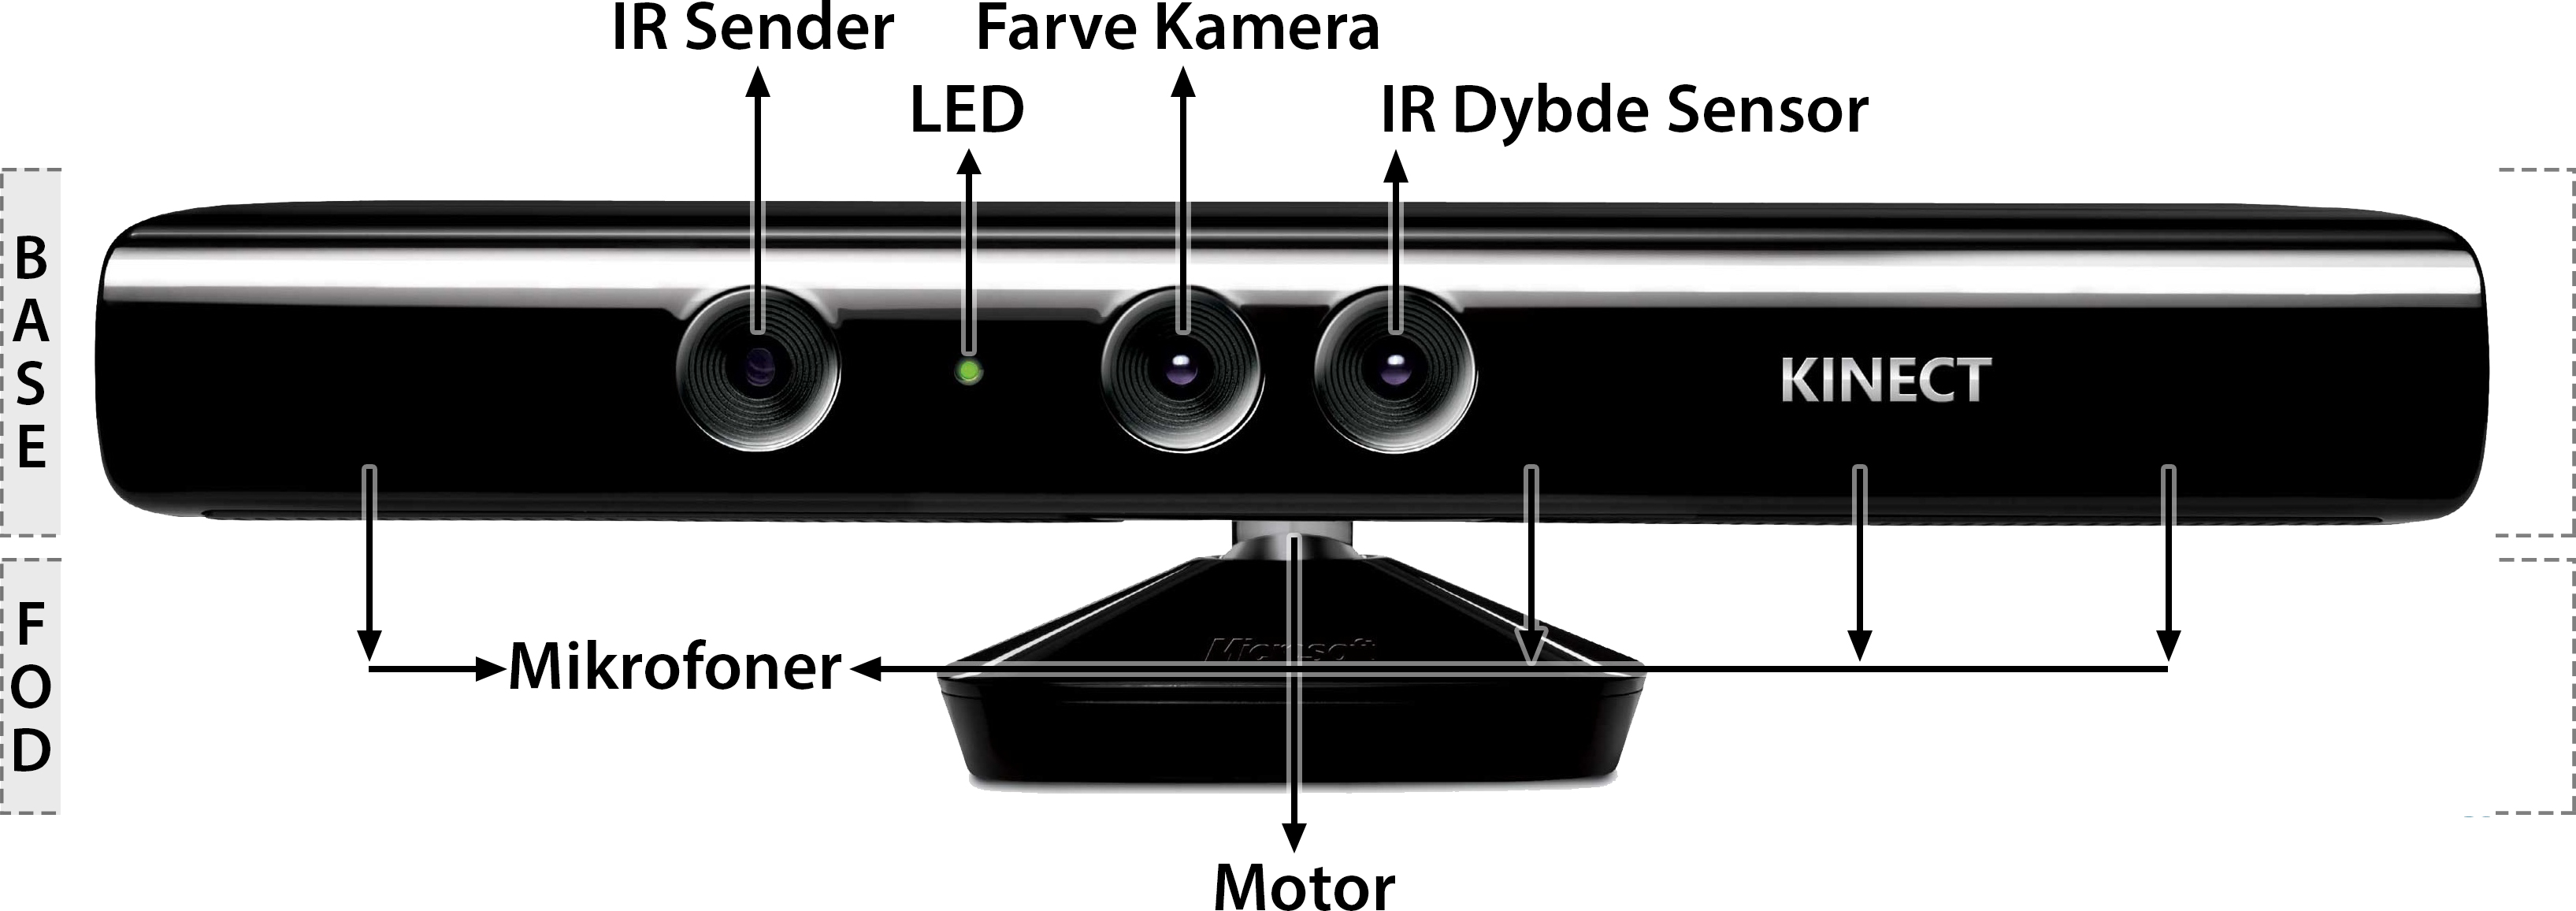
\includegraphics[width=1.0\textwidth]{kinect}
\caption{Opbygning af Microsoft Kinect for Windows}
\label{kinect:opbygning}
\end{figure}

\subsubsection{Farvekamera}
For at gøre Kinecten i stand til at se, er den udstyret med et farvekamera som er placeret ca. i midten.
Et farvekamera kan være nyttigt i spil, hvor man ønsker at vise spilleren fysik på skærmen eller hvis man benytter sin Kinect til gruppechat (som et webcam).
Videoen bliver sendt som en RBG videostrøm med mulighed for en opløsning på 1280x960 med en opdateringshastighed på 12 billeder i sekundet og en lavere opløsning på 640x480 og 30 billeder i sekundet, hvis man ønsker en mere ”flydende” videostrøm\cite{kinectForWindowsFeatures}.

\subsubsection{Infrarød (IR) sender}
Metoden Kinecten benytter for at bestemme personers placeringer og afstanden til dem er vha. infrarøde (IR) signaler der bliver sendt fra en kamera-lignende enhed placeret længst relativ til venstre for de to andre lignende enheder.
Denne enhed udsender infrarødt lys som bliver reflekteret så snart de rammer et objekt i rummet. 
Disse signaler bliver fanget af en anden sensor på Kinecten; nemlig den infrarøde dybde sensor.

Det er også muligt at tilgå det ”rå” infrarøde video signal på samme måde som man kan hente video signalet fra farvekameraet.

\subsubsection{IR dybde sensor}
Når det infrarøde lys bliver reflekteret tilbage mod Kinecten bliver det opfanget af dybde sensoren. 
Når strålerne rammer sensoren bliver informationen konverteret til dybde information, hvori man har en per-pixel afstand til de objekter der er tilstede i billedet.

\subsubsection{Mikrofoner}
Kinecten er også i stand til at optage lyd via de indbyggede mikrofoner.
Dette er dog ikke det eneste mikronfonerne kan benyttes til; de kan også benyttes som en alternativ metode (til dybde billeder) til at bestemme afstand og retning fra f.eks. en person der taler.
Rækken af mikrofoner består af 4 stk som er placeret på fronten af Kinecten.
En mikrofon sidder i venstre side mens de tre andre er placeret til højre på den, hvilket gør det muligt at triangulere lyd signaler for at bestemme retningen af lydkilden.
Flere mikrofoner gør det også muligt at lave ”noise-suppression” ifht. omgivelserne, hvis man benytter Kinect mens man spiller til at kommunikerer med sine med-/modspillere således at unødig støj filtreres fra\cite[s.~15]{kinectProgrammingGuide}.

\subsubsection{Motor til justering af vinklen}
For at gøre det muligt for en Kinect at operere i flere forskellige miljøer og placeringer, er der indbygget en lille motor til at justere vinklen mellem Kinecten og foden den står på.
Den kan bevæge sig fra 0 grader til 27 grader (op) og fra 0 grader til -27 grader (ned).
Bruges Kinecten sammen med en Xbox gør denne detalje det muligt f.eks. at placere den ovenpå eller under fjernsynet.
Med motoren er det også muligt at foretage kalibreringer i real-tid, hvis f.eks. det objekt bevæger sig udenfor synsfeltet.
Dog anbefaler Microsoft at man ikke benytter motoren kontinuært i sine programmer, da den ikke tåler vedvarende belastninger\cite{kinectDocElevationAngle}.

\subsubsection{LED}
Mellem kameraet og IR senderen er der placeret en status LED, der fortæller om driverne dertil at indlæst uden fejl.
Dette kan være nyttigt for udviklere, da det giver sikkerhed for at kommunikationen mellem PC og Kinect er ok\cite[s.~15]{kinectProgrammingGuide}.

\subsubsection{Accelerometer}
Kinect er også udstyret med et 3-akse accelerometer, som udvider den til andre anvendelsesområder end blot at følge (tracke) objekter og kropsbevægelser.
Det er konfigureret til at give målinger fra -2g til 2g (bedre til langsomme bevægelser ifht. højere værdier)\cite{kinectAccelerometer}.
Målingerne  er opbygget som en 3D vektor som peger mod tyngdekraften (gulv-planet), hvilket f.eks. gør det muligt at detektere om den er monteret korrekt (ovenpå eller under et fladskærms tv), således dens tilt kan korrigeres vha. den indbyggede motor.
En anden interessant anvendelsesmulighed er at accelerometeret kan benyttes til at give bedre 3D projektioner i Augmented Reality.
Ifølge dokumentationen\cite{kinectDocAccelerometer} er det præcist ned til en grad, dog med en nøjagtighed der kan varierer med op til 3 grader i forhold til rumtemperaturen.
De skriver endvidere i dokumentationen at der kan kompensateres for denne unøjaghed ved at sammenligne den vertikale måling (y-aksen i accelerometerets koordinatsystem) med den benyttede gulvplans dybde data.


\section{Kinect for Windows SDK}
Da Kinecten udkom fandtes der intet officielt Software Development Kit (SDK) som udviklere kunne bruge til at lave deres egne applikationer til brug på PC\thilemann{gælder det også for Xbox???}, men derimod kun SDK'er udviklet af trediepartsudviklere (der ikke er associeret med Microsoft) som libfreenect (OpenKinect, www.openkinect.org) og OpenNI som er et framework for 3D sensorer (www.openni.org), der skal benyttes med PrimeSense's driver kaldet SensorKinect, for at få adgang til de specifikke data fra sensorene i Kinecten.

\thilemann{måske beskrivelse af windows SDK vs.Libfreekinect og openni?}

Anerledes er det i dag, hvor der findes et officielt SDK (nuværende er version 1,8 – udgivet 17 september, 2013\cite{kinectSDK18}), som åbner op for al funktionalitet i Kinecten med direkte support fra Microsoft.

API'en er bygget op omkring en solid forståelse for menneskers bevægelser og karaktertræk (ikke personlige, men f.eks. hvordan ansigtet er opbygget med næse, øjne og mund samt arme, overkrop og ben) således API'en kan fungere som et interface der kan genkende skeletelle bevægelser, følge ansigter, genkende gestus og tale.
Med Microsoft Kinect Toolkit installeret kan man endvidere få adgang til Microsoft.Kinect.Toolkit namespacet, hvilket indeholder Kinect Fusion som gør det muligt at rekonstruere 3D objekter ud fra Kinectens kamera og dybde information fra IR sensorene.\cite{kinectForWindowsFeatures}


\subsection{Kinect API}
Side 34
Side 49


\subsection{Coding4Fun Kinect Toolkit}


\subsection{Eksempler på brug}
Side 53

\subsubsection{Microsoft.Kinect namespace}

\subsubsection{Coding4Fun.Kinect namespace}

